% ***********************************************************
% ******************* PHYSICS HEADER ************************
% ***********************************************************
% Version 2
\documentclass[12pt]{article}
\usepackage{tikz} % draw automatas
\usetikzlibrary{automata,positioning}
% ***********************************************************
\usepackage{amsmath} % AMS Math Package
\usepackage{amsthm} % Theorem Formatting
\usepackage{amssymb}    % Math symbols such as \mathbb
\usepackage{graphicx} % Allows for eps images
\usepackage[dvips,letterpaper,margin=1in,bottom=0.7in]{geometry}
\usepackage{tensor}
 % Sets margins and page size
\renewcommand{\labelenumi}{(\alph{enumi})} % Use letters for enumerate
% \DeclareMathOperator{\Sample}{Sample}
\let\vaccent=\v % rename builtin command \v{} to \vaccent{}
\usepackage{enumerate}
\renewcommand{\v}[1]{\ensuremath{\mathbf{#1}}} % for vectors
\newcommand{\gv}[1]{\ensuremath{\mbox{\boldmath$ #1 $}}} 
% for vectors of Greek letters
\newcommand{\uv}[1]{\ensuremath{\mathbf{\hat{#1}}}} % for unit vector
\newcommand{\abs}[1]{\left| #1 \right|} % for absolute value
\newcommand{\avg}[1]{\left< #1 \right>} % for average
\let\underdot=\d % rename builtin command \d{} to \underdot{}
\renewcommand{\d}[2]{\frac{d #1}{d #2}} % for derivatives
\newcommand{\dd}[2]{\frac{d^2 #1}{d #2^2}} % for double derivatives
\newcommand{\pd}[2]{\frac{\partial #1}{\partial #2}} 
% for partial derivatives
\newcommand{\pdd}[2]{\frac{\partial^2 #1}{\partial #2^2}} 
% for double partial derivatives
\newcommand{\pdc}[3]{\left( \frac{\partial #1}{\partial #2}
 \right)_{#3}} % for thermodynamic partial derivatives
\newcommand{\ket}[1]{\left| #1 \right>} % for Dirac bras
\newcommand{\bra}[1]{\left< #1 \right|} % for Dirac kets
\newcommand{\braket}[2]{\left< #1 \vphantom{#2} \right|
 \left. #2 \vphantom{#1} \right>} % for Dirac brackets
\newcommand{\matrixel}[3]{\left< #1 \vphantom{#2#3} \right|
 #2 \left| #3 \vphantom{#1#2} \right>} % for Dirac matrix elements
\newcommand{\grad}[1]{\gv{\nabla} #1} % for gradient
\let\divsymb=\div % rename builtin command \div to \divsymb
\renewcommand{\div}[1]{\gv{\nabla} \cdot \v{#1}} % for divergence
\newcommand{\curl}[1]{\gv{\nabla} \times \v{#1}} % for curl
\let\baraccent=\= % rename builtin command \= to \baraccent
\renewcommand{\=}[1]{\stackrel{#1}{=}} % for putting numbers above =
\providecommand{\wave}[1]{\v{\tilde{#1}}}
\providecommand{\fr}{\frac}
\providecommand{\RR}{\mathbb{R}}
\providecommand{\NN}{\mathbb{N}}
\providecommand{\seq}{\subseteq}
\providecommand{\e}{\epsilon}

\newtheorem{prop}{Proposition}
\newtheorem{thm}{Theorem}[section]
\newtheorem{axiom}{Axiom}[section]
\newtheorem{p}{Problem}[section]
\usepackage{cancel}
\newtheorem*{lem}{Lemma}
\theoremstyle{definition}
\newtheorem*{dfn}{Definition}
 \newenvironment{s}{%\small%
        \begin{trivlist} \item \textbf{Solution}. }{%
            \hspace*{\fill} $\blacksquare$\end{trivlist}}%
% ***********************************************************
% ********************** END HEADER *************************
% ***********************************************************

\begin{document}

{\noindent\Huge\bf  \\[0.5\baselineskip] {\fontfamily{cmr}\selectfont  Problem Set I}         }\\[2\baselineskip] % Title
{ {\bf \fontfamily{cmr}\selectfont Computing Models}\\ {\textit{\fontfamily{cmr}\selectfont     April 23, 2023}}}~~~~~~~~~~~~~~~~~~~~~~~~~~~~~~~~~~~~~~~~~~~~~~~~~~~~~~~~~~~~~~~~~~~~~~~~~~~~~    {\large \textsc{Alon Filler}\footnote{With $\Sigma$orer}} % Author name
\\[1.4\baselineskip] 



\section{Finite Deterministic Automatas}
\emph{Given the automata $D = (Q^{D}, \{a,b\}, \delta^{D}, q_0^{D}, F^{D})$} \newline
\begin{p}
\emph{\newline Imagine a new automata $E = (Q^{E}, \{a,b\}, \delta^{E}, q_0^{E}, F^{E})$} s.t:
\begin{itemize}
  \item $Q^{E} = Q^{D} \cup \{q_0^{E}\}$
  \item $F^{E} = F^{D}$
  \item \(
    \hspace{0mm}
    \delta^{E}(q, \sigma) = 
    \begin{cases}
      \delta^{D}(q, \sigma) & q \in Q^{D} \\
        q_0^{D} & q = q_0^{E}, \sigma = a \\ 
        q_0^{E} & q = q_0^{E}, \sigma = b
    \end{cases}
  \)
\end{itemize}

Define: 
\begin{itemize}
  \item L(A)
\end{itemize}
\end{p}
\begin{s} \newline
\emph{It would be non but rational to divide this construction into three divisions, each corresponding to a different set of circumstances recognised by the trasitions function.} \newline
\\
\emph{One of those aforementioned circumstances is $q = q_0^{E}, \sigma = b$, the study of such case lead me to determine that for the character input of b, under the assumption that the current state is $q_0^{E}$, the state would lead back to itself, meaning that that an instance of $\{b\}^{*}$ at the beginning of the input would not affect the output of the automata. And hence $\{b\}^{*}$ should be imbued to the language L(A).} \newline
\\
\emph{Another set of circumstances is $q = q_0^{E}, \sigma = a$, which implies the current state to be the one added to $Q^{D}$ in order to craft $Q^{E}$, and that the input chracter is 'a'. Such circumstances appear to be digested by the automata to return $q_0^{D}$, the first state of the previous automata D. Accordingly, it would only be after the appearence of an 'a' character in the input that the state would be changed. And hence, $\{a\}$ must be added to the language L(A).} \newline
\\
\emph{The last of such circumstances addressed in $\delta^{E}$ appears to be $q \in Q^{D}$. For such case, the function would make the transition from the current state to the one returned by $\delta^{D}$, accordingly, L(D) must be concatenated at the end of L(E)} \newline 
\\
\emph{Hence - I may declare that $L(A) = \{b\}^{*} \cdot \{a\} \cdot L(D)$.}
\end{s}
\begin{p}
  \emph{\newline Consider the previous automata\footnote{Problem 1.1} $E = (Q^{E}, \{a,b\}, \delta^{E}, q_0^{E}, F^{E})$} \newline
  \emph{And a new automata $E^{\prime} = (Q^{E}, \{a,b\}, \delta^{E}, q_0^{D}, F^{E})$} \newline
  \\
  Define: 
  \begin{itemize}
    \item $L(E^{\prime})$
  \end{itemize}
\end{p}
\begin{s} \newline
  \emph{In the previous problem\footnote{Problem 1.1} I have explained in great detail the effects caused by the declaration of a new state $q_0^{E}$ to be the initial state of E. Considering $q_0^{E}$ not to be part of $Q^{D}$, it can be seen with vividness that $\delta^{E}$, known as $E^{\prime}$'s transitions function would cease to return it as output as soon as it no longer is the current state. Therefore, knowing $E^{\prime}$ does not use $q_0^{E}$ as its initial state it is cogent that it would never be returned. Accordingly, the only circumstances relevant to the transitions function would be $q \in Q^{D}$, and thus the addition of $\{b\}^{*} \cdot \{a\}$ to the beginning of L(E) must be undone for $L(E^{\prime})$ to be precise. And hence $L(E^{\prime}) = L(D)$}
\end{s}
\begin{p}
  \emph{\newline Consider the previous automata\footnote{Problem 1.2} $E = (Q^{E}, \{a,b\}, \delta^{E}, q_0^{E}, F^{E})$} \newline
  \emph{And a new automata $E^{\prime} = (Q^{E}, \{a,b\}, \delta^{E}, q_0^{D}, F^{D} \cup q_0^{E})$} \newline
  \\
  Define: 
  \begin{itemize}
    \item $L(E^{\prime})$
  \end{itemize}
\end{p}
\begin{s} \newline
  \emph{Now that $q_0^{E}$ is an accepting state, I should like for $L(E^{\prime})$ to support it. Thus, anything that happens to follow $\{b\}^{*}$ is merely optional. And hence it might be defined as such: $L(E^{\prime}) = \{b\}^{*} \cdot \{\{\epsilon\} \cup (\{a\} \cdot L(D))\}$} 
\end{s}
  \emph{\newline Consider the previous automata\footnote{Problem 1.1} $E = (Q^{E}, \{a,b\}, \delta^{E}, q_0^{E}, F^{E})$} \newline
\newpage
\section{Finite Non Deterministic Automatas}
\begin{p}
  \emph{\newline Build an automata to accept a language above $\{0,1\}$ where each word is terminated with a character that follows a 0.} \newline
\end{p}
\begin{s} \newline
 \emph{The automata should have states, three in number, an initial one to which the automata would never appoint once departed from, one to acknowledge the preceding zero and one to halt upon receiving redundant input.} \newline
  \\
  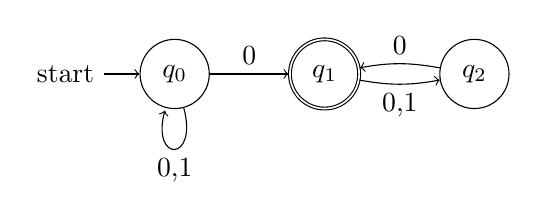
\begin{tikzpicture}
    \node [state, initial] (q_0) {$q_0$};
    \node [state, accepting] [right=of q_0] (q_1) {$q_1$};
    \node [state] [right=of q_1] (q_2) {$q_2$};
      \path[->]
      (q_0) edge [loop below] node [below] {{0,1}} ()
      (q_0) edge node [above] {0} (q_1)
      (q_1) edge [bend right=10] node [above=0.25] {0} (q_2)
      (q_2) edge [bend right=10] node [below=0.25] {{0,1}} (q_1)
      ;
  \end{tikzpicture}
\end{s}
\begin{p}
  \emph{\newline Build an automata to accept a language above $\{0,1\}$ where each word contains the string 1101.} \newline
\end{p}
\begin{s} \newline
 \emph{The automata should have four states, each corresponding to a letter of the string 1101 and an additional one to process redundant input. Considering the automata not to be deterministic, it may be assumed that upon shifting from the initial state, the only characters to follow would be 101 and so on and so forth for the next characters.} \newline
  \\
  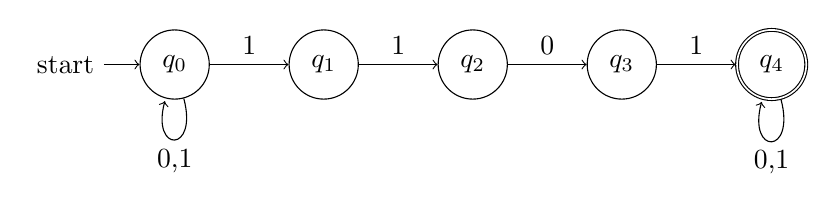
\begin{tikzpicture}
    \node [state, initial] (q_0) {$q_0$};
    \node [state] [right=of q_0] (q_1) {$q_1$};
    \node [state] [right=of q_1] (q_2) {$q_2$};
    \node [state] [right=of q_2] (q_3) {$q_3$};
    \node [state, accepting] [right=of q_3] (q_4) {$q_4$};
      \path[->]
      (q_0) edge [loop below] node [below] {{0,1}} ()
      (q_0) edge node [above] {1} (q_1)
      (q_1) edge node [above] {1} (q_2)
      (q_2) edge node [above] {0} (q_3)
      (q_3) edge node [above] {1} (q_4)
      (q_4) edge [loop below] node [below] {{0,1}} ()
      ;
  \end{tikzpicture}
\end{s}
\end{document}
